%Title: Fus. evap results for U and Th isotopes
%Author: A. Raggio
%Year: 2020

\documentclass[10pt]{beamer}

%
%Setting file
%

\usepackage[T1]{fontenc}
\usepackage[utf8]{inputenc}

\usepackage[english]{babel}

\usepackage{graphicx}
\graphicspath{{images/}}
\usepackage{float}
\usepackage{tikz}
\usepackage{caption}
\usepackage{subcaption}

\usetheme{default}
\usefonttheme{structurebold}


% ---------------------------------
% color definitions
\usepackage{color}
% \definecolor{LISA_BLUE}{rgb}{0.25,0.33,0.66}
\definecolor{LISA_BLUE}{cmyk}{0.99,0.88,0.29,0.18}

\setbeamercolor{normal text}{fg=LISA_BLUE}
\setbeamercolor{frametitle}{fg=LISA_BLUE}

\newcommand\insertlocation{}  % Empty by default.
\newcommand\location[1]{\renewcommand\insertlocation{#1}}

\newcommand\insertperiod{}  % Empty by default.
\newcommand\period[1]{\renewcommand\insertperiod{#1}}



\setbeamertemplate{itemize items}[circle]
\setbeamercolor{title}{fg=white}



%-----------------------------------------Title page settings-----------------------------------------%
\title{ESR 4}
\subtitle{Introduction}
\author{Andrea Raggio}
\institute{Department of Physics\\University of Jyv\"askyl\"a}
\period{November 2020}
\location{Mid-Term Review}


\date{}

%-----------------------------------------Title page settings-----------------------------------------%


% \setbeamertemplate{footline}
% {
%  \begin{beamercolorbox}{section in head/foot}
%  \vskip2pt\hspace{0.095cm} Andrea Raggio \hfill Jyv\"{a}skyl\"{a} - 13 November 2020 \hspace{0.15cm}\phantom{x}\vskip2pt
%  \end{beamercolorbox}%
% }


\begin{document}

{
  \usebackgroundtemplate{
\includegraphics[width=\paperwidth]{Title.pdf}}
	\begin{frame}[noframenumbering, plain]
		\titlepage
	\end{frame}
}

\begin{frame}{Where}
	\centering
	\only<1>{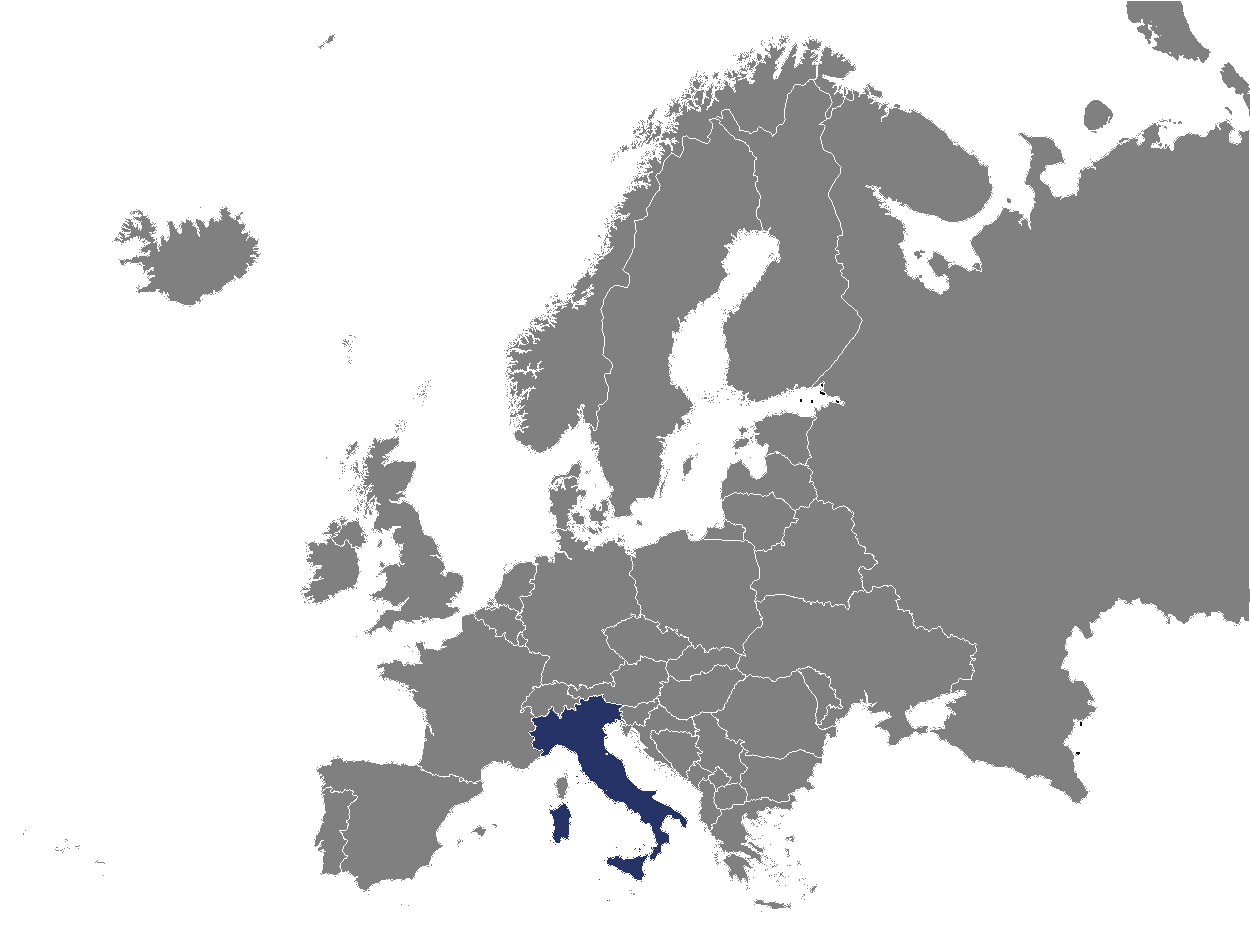
\includegraphics[width=0.9\textwidth]{map_0.pdf}}%
	\only<2>{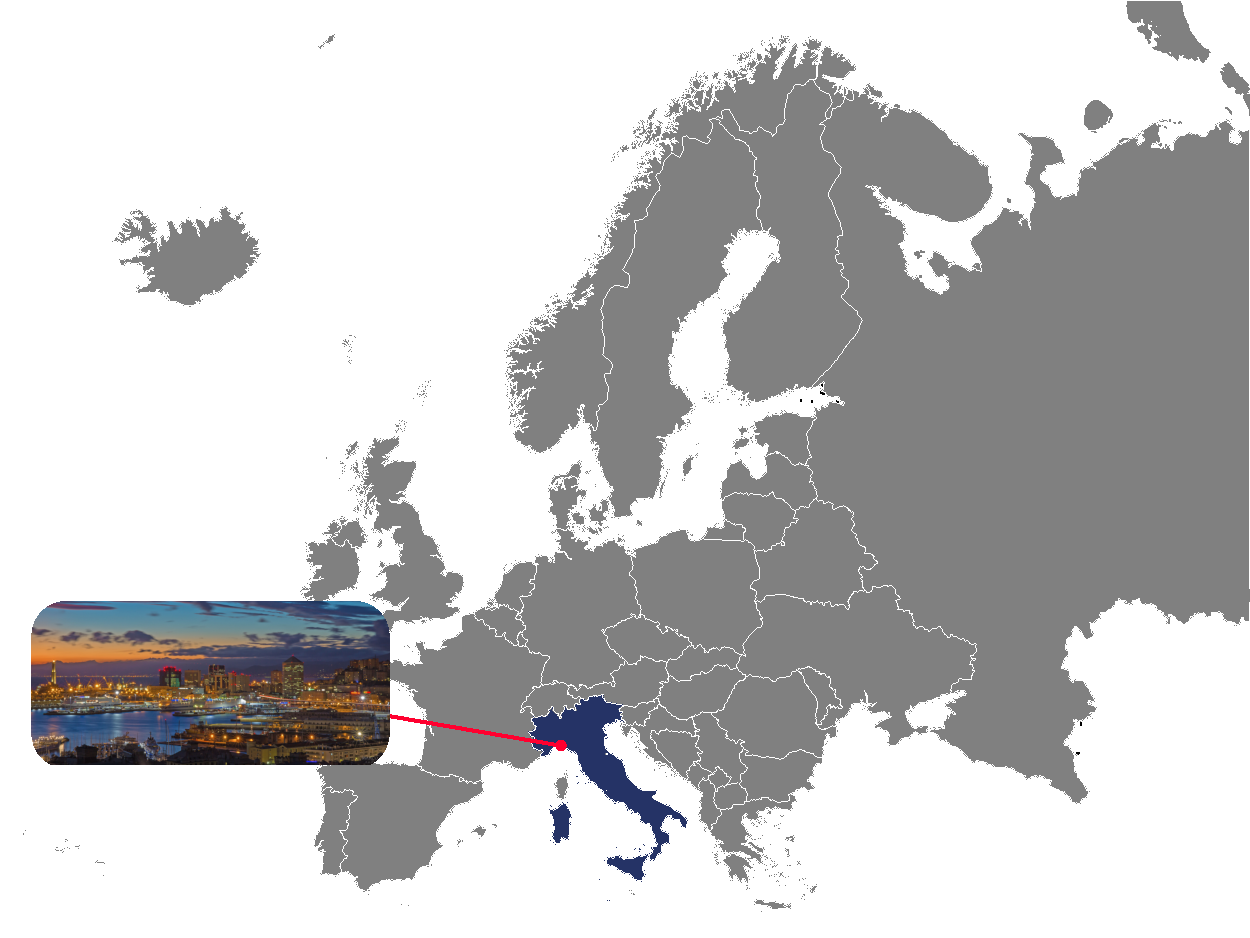
\includegraphics[width=0.9\textwidth]{map_1.pdf}}%
	\only<3>{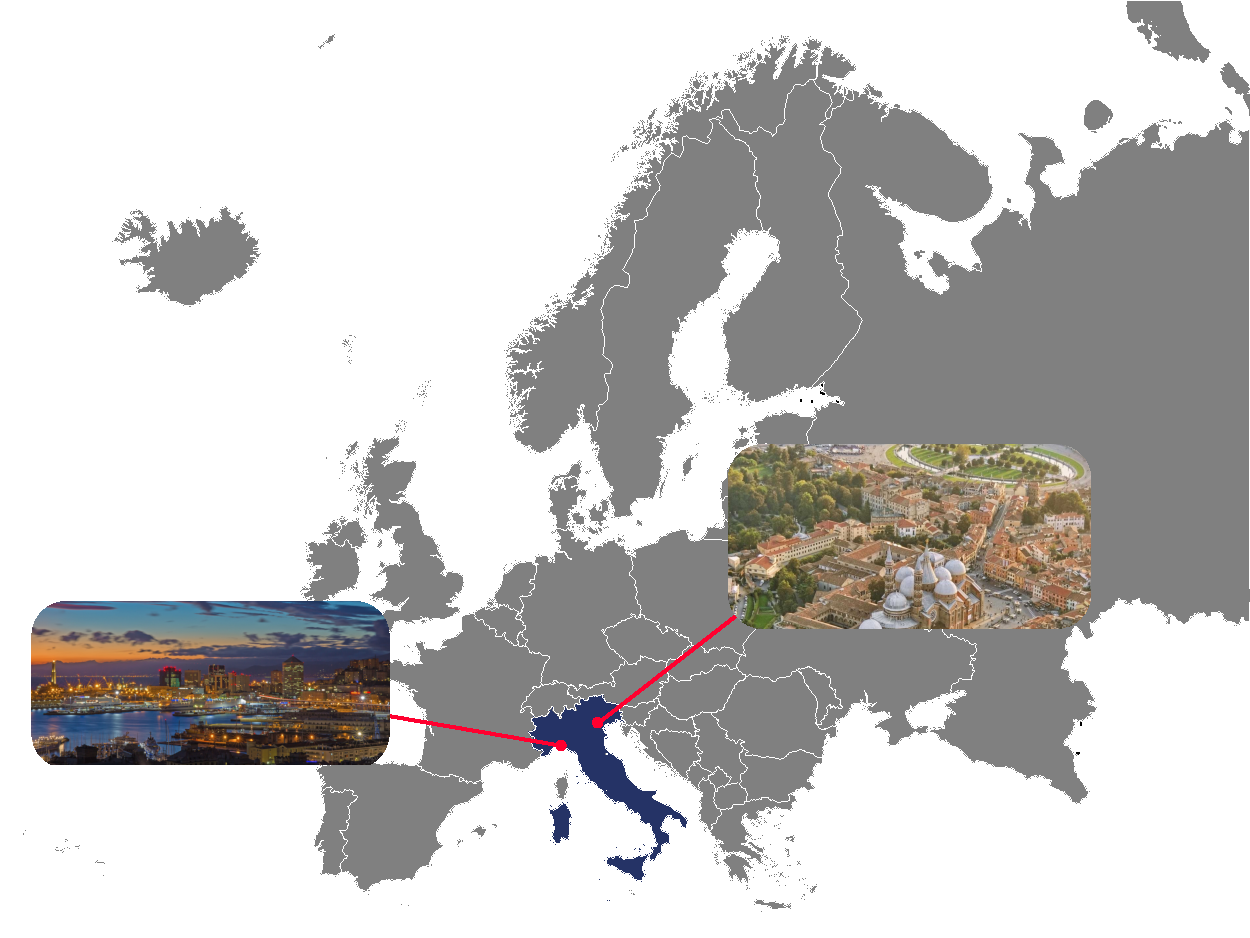
\includegraphics[width=0.9\textwidth]{map_2.pdf}}%
	\only<4>{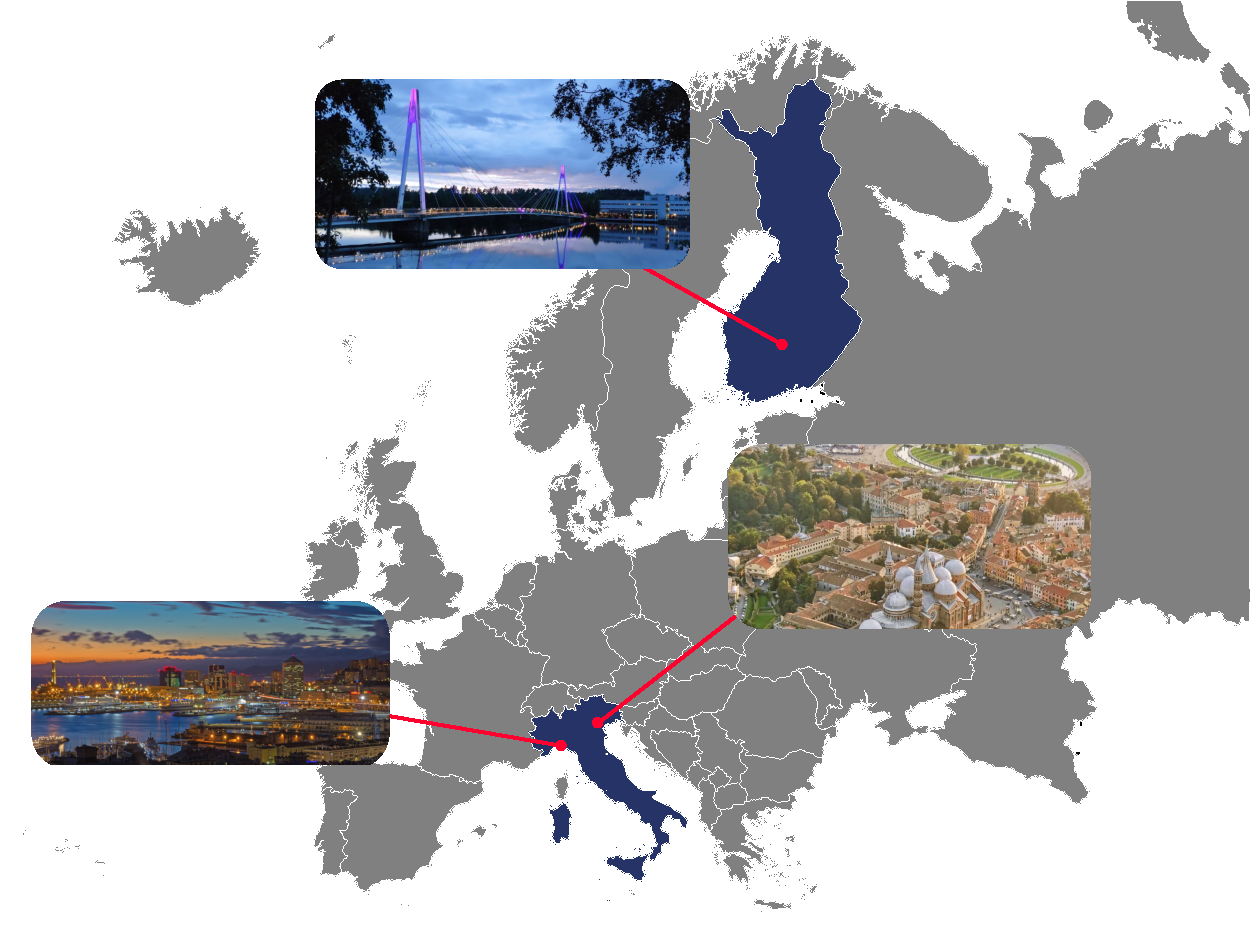
\includegraphics[width=0.9\textwidth]{map_3.pdf}}%
\end{frame}

\begin{frame}{\small High-resolution laser spectroscopy of actinide elements for nuclear structure}
	\begin{columns}
		\begin{column}{0.5\textwidth}
			\begin{overlayarea}{\textwidth}{\textheight}
				\centering
				\vspace{0.05\textheight}
				\textbf{WP5}\\ Exploring the limits of nuclear existence 		
				\begin{itemize}
					\item<2-> Decay modes and lifetime
					\item<3-> Nuclear spins\\ electromagnetic moments\\ mean-square charge radii
					\item<4-> Actinide Target preparation 
					\item<5-> Laser spectroscopy on SHE\\ Exploitation of gas-jet environment 
				\end{itemize}
			\end{overlayarea}
		\end{column}
		\begin{column}{0.6\textwidth}
			\begin{overlayarea}{\textwidth}{\textheight}
				\vspace{0.05\textheight}
				\textbf{I}on \textbf{G}uide \textbf{I}sotope \textbf{S}eparation \textbf{O}n-\textbf{L}ine
				\centering
				\only<1>{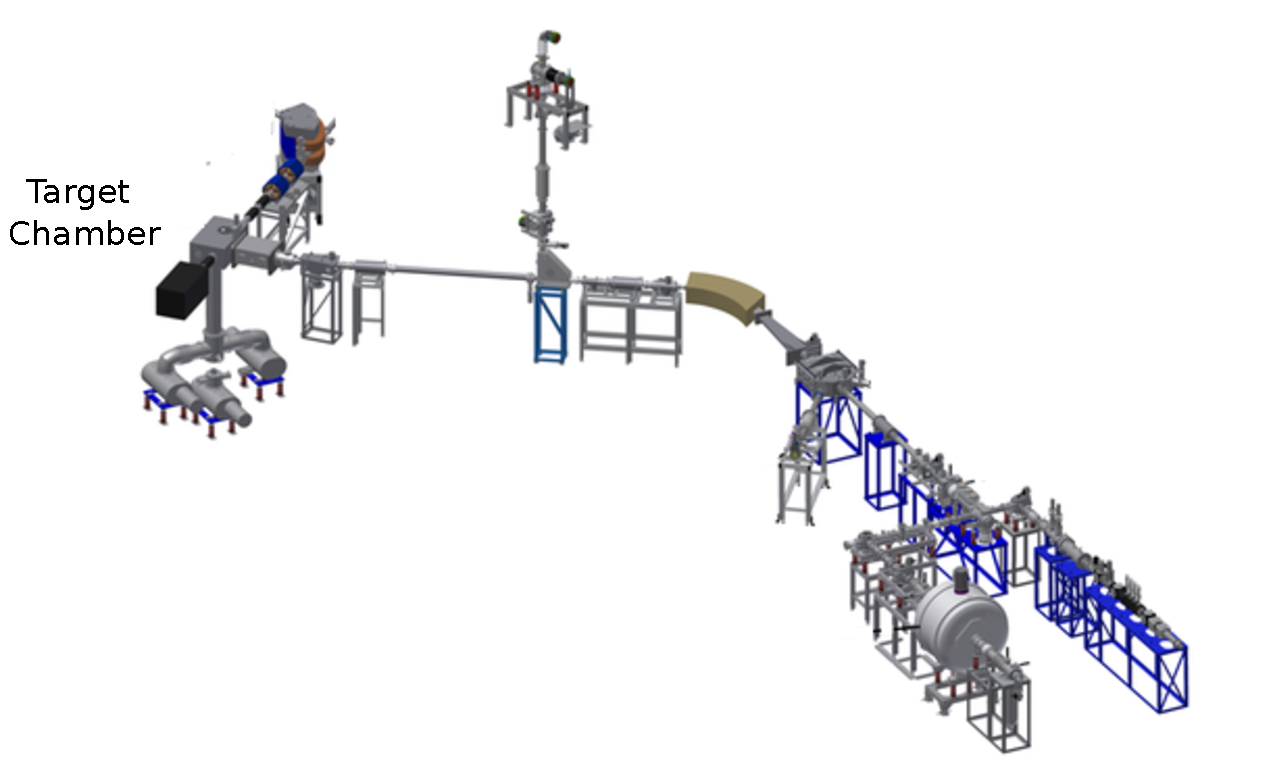
\includegraphics[width=0.9\textwidth]{igisolscheme_1.pdf}}%
				\only<2>{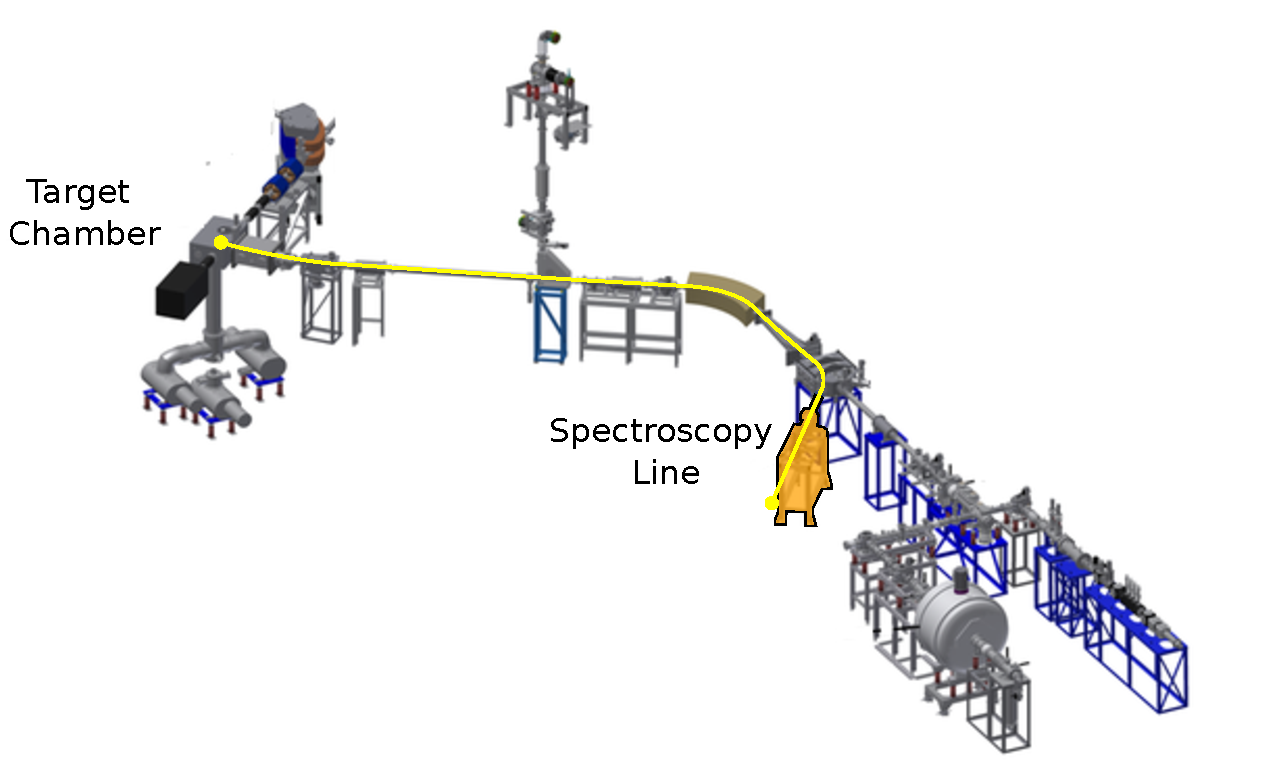
\includegraphics[width=0.9\textwidth]{igisolscheme_2.pdf}}%
				\only<3->{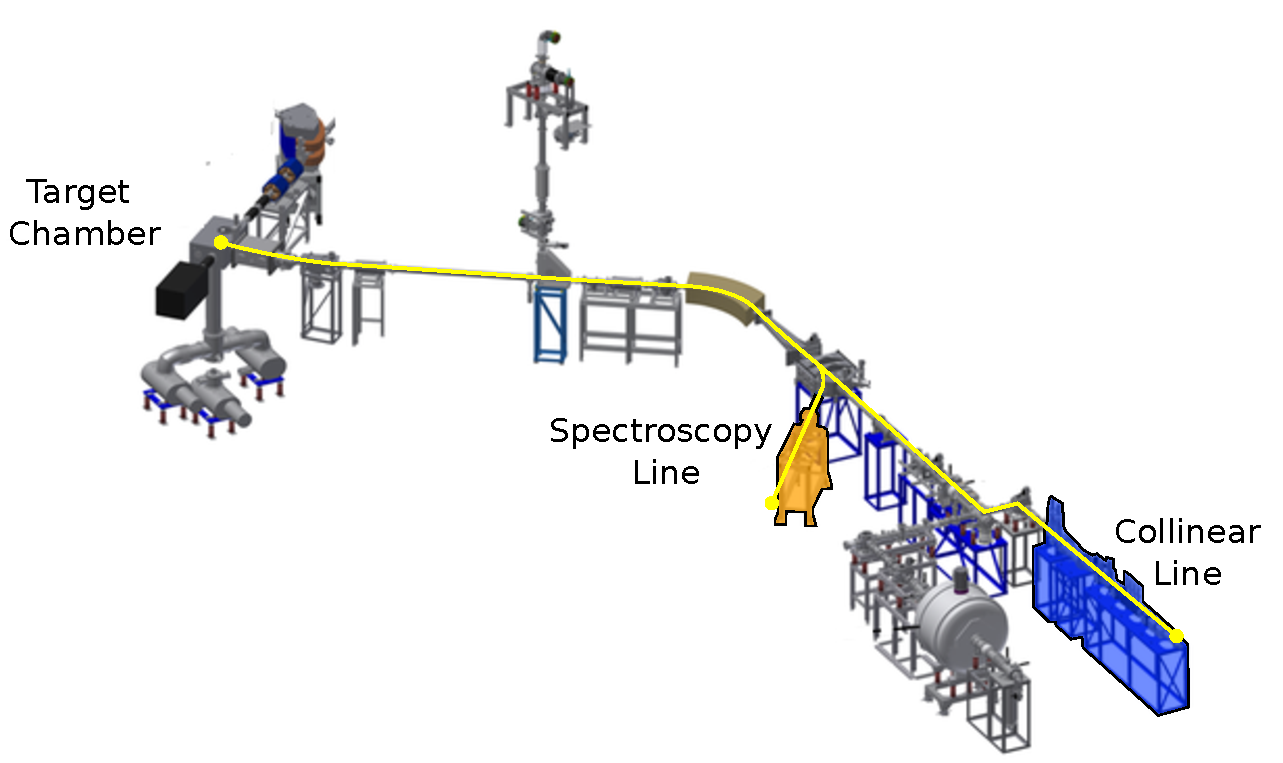
\includegraphics[width=0.9\textwidth]{igisolscheme_4.pdf}}\\%
				\visible<4->{
\includegraphics[width=0.4\textwidth]{Mainz.png}}\\%
				\visible<5>{
\includegraphics[width=0.4\textwidth]{GSI_Logo.png}}%

			\end{overlayarea}
		\end{column}
	\end{columns}
	

\end{frame}


\end{document}
